\chapter[Doing tomography based on the sensitivity kernels obtained]{Doing tomography, i.e., updating the model based on the sensitivity kernels obtained}\label{cha:tomo}

UNDER CONSTRUCTION (July 2015). New content will be added soon.

\section{Tomographic full waveform inversion (FWI) / imaging using the sensitivity kernels obtained}

One of the fundamental reasons for computing sensitivity kernels (Section~\ref{sec:Adjoint-simulation-finite})
is to use them within a tomographic inversion, i.e., perform imaging. In other words, use
recorded seismograms, make measurements with synthetic seismograms,
and use the misfit between the two to iteratively improve the model
described by (at least) $V_{{\rm p}}$, $V_{{\rm s}}$, and $\rho$ as a function of space.

As explained for instance in \cite{MoChKoWa15},
full waveform inversion means that one considers the observed seismograms (possibly filtered) as the
basic observables that one wants to fit. One thus searches for the model that minimizes the mean squared difference between observed
and synthetic seismograms. In other words, the goal is to find a structural model that can explain a larger portion
of seismological records, and not simply the phase of a few seismic arrivals.

Whatever misfit function you use for the tomographic inversion (you can find several
examples in \citet{TrKoLi08} and \citet{TrTaLi05}), you will weigh
the sensitivity kernels with measurements. Furthermore, you will use
as many measurements (stations, components, time windows) as possible
per event; hence, we call these composite kernels ``event kernels'',
which are volumetric fields representing the gradient of the misfit
function with respect to one of the variables (\eg $V_{{\rm s}}$).
The basic features of an adjoint-based tomographic inversion were
illustrated in \citet{TrKoLi08} and \citet{TaLiTr07} using a conjugate-gradient algorithm.
Other, more powerful techniques such as the Limited-Memory Broyden-Fletcher-Goldfarb-Shanno (L-BFGS) method can now be used,
as illustrated for instance in \cite{MoChKoWa15}.

\subsection{Principle}

We want to minimize the classical waveform misfit function:
\begin{equation}
\chi \left( \boldm \right) = \sum_{s=1}^N\sum_{r=1}^M \int_0^T \frac{1}{2} \|\boldu(\boldx_r, \boldx_s; t) - \boldd(\boldx_r, \boldx_s; t)\| ^{2} \, dt .
\label{misfit}
\end{equation}
This functional quantifies the $L^2$ difference between the observed waveforms $\boldd(\boldx_r, \boldx_s; t)$ at receivers $\boldx_r$, $r = 1, ..., M$
produced by sources at $\boldx_s$, $s=1,...,N$, and the corresponding synthetic seismograms $\boldu(\boldx_r, \boldx_s; t)$ computed in model $\boldm$.
While this misfit function is indeed classical, it is worth mentioning that in the case of noisy real data other norms could be used,
since in the oil industry for instance it is known that the $L^1$ norm
(\cite{CrPiNoMcTa90,BrOpVi2010}), hybrid $L^1-L^2$ norms (\cite{Bube_1997_HL1}), Hubert norm (\cite{Ha_2009_WIU}),
Student-t distribution (\cite{ArVaHe11,Jeong_2015}) etc... can be more robust that the $L^2$ norm used here in the context of synthetic data with no noise.
In the vicinity of $\boldm$, the misfit function can be expanded into a Taylor series:
\begin{equation}
\chi(\boldm+ \delta\boldm) \approx \chi(\boldm)+\boldg(\boldm)\cdot\delta\boldm
+\delta\boldm\cdot\mathbf{H}(\boldm)\cdot\delta\boldm \, ,
\label{local_misfit}
\end{equation}
where $\boldg(\boldm)$ is the gradient of the waveform misfit function:
\begin{equation}
\boldg(\boldm) = \frac{\partial\chi(\boldm)}{\partial\boldm} \, ,
\end{equation}
and $\mathbf{H}(\boldm)$ the Hessian:
\begin{equation}
\mathbf{H}(\boldm) = \frac{\partial^2\chi(\boldm)}{\partial\boldm^2} \, .
\end{equation}
In the following, for simplicity the dependence of the gradient and Hessian on the model will be implicitly assumed and omitted in the notations.
The nearest minimum of $\chi$ in (\ref{local_misfit}) with respect to the model perturbation $\delta \boldm$ is reached for
\begin{equation}
\delta \boldm = -\mathbf{H}^{-1} \cdot \boldg \, .
\label{Newton}
\end{equation}
The local minimum of (\ref{misfit}) is thus given by perturbing the model in the direction of the gradient preconditioned
by the inverse Hessian.

\subsection{Computation of the gradient based on the adjoint method}

A direct method to compute the gradient is to take the derivative of (\ref{misfit}) with respect to model parameters:
\begin{equation}
\frac{\partial\chi(\boldm)}{\partial\boldm} = -\sum_{s=1}^N\sum_{r=1}^M \int_0^T
\frac{\partial \boldu(\boldx_r, \boldx_s; t)}{\partial\boldm}\cdot\left[\boldu(\boldx_r, \boldx_s; t) - \boldd(\boldx_r, \boldx_s; t)\right] \, dt \, .
\label{calc_gradient}
\end{equation}
This equation can be reformulated as the matrix-vector product:
\begin{equation}
\boldg = -\mathbf{J}^* \cdot \delta \mathbf{d} \, ,
\label{Jacobian}
\end{equation}
where $\mathbf{J}^*$ is the adjoint of the Jacobian matrix of the forward problem that contains the Fr\'echet derivatives of the
data with respect to model parameters, and $\delta \mathbf{d}$ is the vector that contains the data residuals.
The determination of $\mathbf{J}$ would require computing the Fr\'echet derivatives for each time step in the time
window considered and for all the source-station pairs, which is completely prohibitive on current supercomputers
(let us note that this situation may change one day).
However, it is possible to obtain this gradient without computing the Jacobian matrix explicitly.
The approach to determine the gradient without computing the Fr\'echet derivatives was introduced in nonlinear optimization
by \cite{Cha74} working with J. L. Lions, and later applied to seismic exploration problems by
\cite{BaChLa77}, \cite{BaChHeLa82}, \cite{Lai83} and \cite{Tar84}. The idea is to resort to the adjoint state,
which corresponds to the wavefield emitted and back-propagated from the receivers \cite[e.g.,][]{TrTaLi05,TrKoLi08,Plessix_2006_RAS,FiBuIg06}.

Let us give an outline of the theory to compute the gradient based on the adjoint method, and refer the reader to e.g. \cite{TrTaLi05}
and \cite{TrKoLi08} for further details. The perturbation of the misfit function can be expressed as:
\begin{equation}
\delta \chi (\boldm) = \sum_{s=1}^N\sum_{r=1}^M \int_0^T \left[\boldu(\boldx_r, \boldx_s; t) - \boldd(\boldx_r, \boldx_s; t)\right]\cdot \delta
\boldu(\boldx_r, \boldx_s; t) \, dt \, ,
\label{dchi}
\end{equation}
where $\delta\boldu$ is the perturbation of displacement given by the first-order Born approximation \cite[e.g.,][]{Hud77}:
\begin{eqnarray}
\delta \boldu (\boldx_r, \boldx_s; t) & = & -\int_0^t \int_V
\left[\delta\rho(\boldx)\mathbf{G}(\boldx_r,\boldx;t-t')\cdot\partial^2_{t'}\boldu(\boldx,\boldx_s;t') \right. \nonumber \\
& + & \left. \nabla \mathbf{G}(\boldx_r,\boldx;t-t'):\delta \boldc(\boldx): \nabla\boldu(\boldx;t') \right] \, d^3\boldx \, dt' \, .
\label{Born}
\end{eqnarray}
In this expression, $\mathbf{G}$ is the Green's tensor, $\delta\rho$ the perturbation of density, $\delta c$ the perturbation of the fourth-order elasticity
tensor,
and a colon denotes a double tensor contraction operation.
Inserting (\ref{Born}) into (\ref{dchi}) we obtain
\begin{eqnarray}
\delta \chi (\boldm) & = & -\sum_{s=1}^N\sum_{r=1}^M \int_0^T \left[\boldu(\boldx_r, \boldx_s; t) - \boldd(\boldx_r, \boldx_s; t)\right] \int_0^t \int_V
\left[\delta\rho(\boldx)\mathbf{G}(\boldx_r,\boldx;t-t')\cdot\partial^2_{t'}\boldu(\boldx,\boldx_s;t') \right. \nonumber \\
& + & \left. \nabla \mathbf{G}(\boldx_r,\boldx;t-t'):\delta \boldc(\boldx):\nabla\boldu(\boldx,t') \right] \, d^3\boldx \, dt' \, dt \,.
\end{eqnarray}
Defining the waveform adjoint source for each source $\boldx_s$
\begin{equation}
\boldf^\dagger(\boldx,\boldx_s;t) = \sum_{r=1}^M  \left[\boldu(\boldx_r, \boldx_s; T-t) - \boldd(\boldx_r, \boldx_s; T-t)\right] \delta(\boldx-\boldx_r) \, ,
\end{equation}
and the corresponding adjoint wavefield
\begin{equation}
\boldu^\dagger(\boldx,\boldx_s;t) = \int_0^{t'}\int_V\mathbf{G}(\boldx,\boldx';t'-t)\cdot\boldf^\dagger(\boldx',\boldx_s;t)\, d^3\boldx' \, dt \, ,
\end{equation}
the perturbation of the misfit function may be expressed as:
\begin{eqnarray}
\delta\chi(\boldm) & = & - \sum_{s=1}^N\nonumber \int_V \int_0^T \left[\delta\rho \, \boldu^\dagger(\boldx,\boldx_s;T-t)\cdot
\partial^2_{t}\boldu(\boldx,\boldx_s;t) \right. \nonumber \\
& +  & \left. \nabla\boldu^\dagger(\boldx,\boldx_s;T-t):\delta \boldc: \nabla \boldu(\boldx,\boldx_s;t) \right] \, d^3\boldx \, dt \, .
\label{dchi2}
\end{eqnarray}
At this point, we make some assumptions on the nature of the elasticity tensor.
A general fourth-order elasticity tensor is described by 21 elastic parameters, a very large number that makes its complete characterization
way beyond the reach of any tomographic approach. For the time being, let us thus consider isotropic elasticity tensors,
described by the two Lam\'e parameters $\lambda$ and $\mu$:
\begin{equation}
c_{ijkl} = \lambda \delta_{ij}\delta_{kl}+\mu(\delta_{ik}\delta_{jl}+\delta_{il}\delta_{jk}) \, .
\end{equation}
In this case, (\ref{dchi2}) can be written as:
\begin{eqnarray}
\delta\chi(\boldm) & = & - \sum_{s=1}^N\nonumber \int_V \left[ K_\rho(\boldx,\boldx_s)\delta\ln\rho(\boldx)
+K_\lambda(\boldx,\boldx_s)\delta\ln\lambda(\boldx) \right. \nonumber \\
& + & \left. K_\mu(\boldx,\boldx_s)\delta\ln\mu(\boldx)\right] \, d^3\boldx \, ,
\label{dchi2_1}
\end{eqnarray}
where ln() is the natural logarithm and where the Fr\'echet derivatives with respect to the density and Lam\'e parameters are given by:
\begin{eqnarray}
K_\rho(\boldx,\boldx_s) & = & - \int_0^T \rho(\boldx) \boldu^\dagger(\boldx,\boldx_s;T-t)\cdot \partial^2_{t}\boldu(\boldx,\boldx_s;t) \, dt \\
K_\lambda(\boldx,\boldx_s) & = & - \int_0^T \lambda(\boldx) \nabla\cdot\boldu^\dagger(\boldx,\boldx_s;T-t) \nabla\cdot\boldu(\boldx,\boldx_s;t) \, dt \\
K_\mu(\boldx,\boldx_s) & = & -2 \int_0^T \mu(\boldx) (\boldx) \nabla\boldu^\dagger(\boldx,\boldx_s;T-t) :\nabla\boldu(\boldx,\boldx_s;t)\, dt \, .
\end{eqnarray}
Since the propagation of seismic waves mainly depends on compressional wave speed $\alpha$ and shear wave speed $\beta$,
but also because these seismic velocities are easier to interpret, tomographic models are usually described based on these
two parameters. With this new parametrization, the perturbation of the misfit function may be written as:
\begin{eqnarray}
\delta\chi(\boldm) & = & - \sum_{s=1}^N\nonumber \int_V \left[ K'_\rho(\boldx,\boldx_s)\delta\ln\rho(\boldx)
+K'_\alpha(\boldx,\boldx_s)\delta\ln\alpha(\boldx) \right. \nonumber \\
& + & \left. K'_\beta(\boldx,\boldx_s)\delta\ln\beta(\boldx)\right] \, d^3\boldx \, ,
\end{eqnarray}
where
\begin{eqnarray}
K'_\rho(\boldx,\boldx_s) & = &  K_\rho(\boldx,\boldx_s)+K_\lambda(\boldx,\boldx_s)+K_\mu(\boldx,\boldx_s) \\
K'_\alpha(\boldx,\boldx_s) & = &  2 \left(\frac{\lambda+2\mu}{\lambda}\right) K_\lambda(\boldx,\boldx_s) \\
K'_\beta(\boldx,\boldx_s) & = & 2 K_\mu -\frac{4\mu}{\lambda} K_\lambda (\boldx,\boldx_s) \, .
\end{eqnarray}

As can be seen from these expressions, the principle of the adjoint-state method is to correlate two wavefields:
the direct (i.e. forward) field that propagates from the source to the receivers, and the adjoint field that propagates from all the
receivers backward in time. The same approach can be followed for any type of seismic observable (phase, amplitude,
envelope, time series...), provided the appropriate adjoint source is used \cite[]{TrTaLi05,TrKoLi08}.
For example, for the cross-correlated traveltime of a seismic
phase, the adjoint source is defined as the velocity of that synthetic phase weighted by the travel-time residual.

Computing the gradient based on the adjoint-state method requires performing two simulations per source (forward and adjoint
fields) regardless of the type of observable. However, to define the adjoint field one
must know the adjoint source, and that source is computed from the results of the forward simulation. One must therefore perform
the forward simulation before the adjoint simulation.
A straightforward solution for time-domain methods would be to store the whole forward field to disk at
each time step during the forward run and then read it back during the adjoint simulation to calculate the interaction of these two fields.
In 2-D this is feasible but in the 3-D case for very short seismic periods and without lossy compression, downsampling,
or a large amount of disk or memory checkpointing \cite[e.g.,][]{FiKeIg09,RuHaPuGu14,CyShWi15}
the amount of disk storage required would currently be too large.

However let us note again that this situation will change in the future.
In the mean time, a standard possible solution is to perform three simulations per source \cite[]{TrKoLi08,PeKoLuMaLeCaLeMaLiBlNiBaTr11},
i.e., perform the forward calculation twice, once to compute the adjoint sources and once again
at the same time as the adjoint simulation to correlate the two fields and sum their interaction on the fly over all the time steps.
Doing so for an elastic Earth, one only needs a small amount of disk storage to store the last time
step of the forward run, which is then used as an initial condition to redo the forward run backwards,
as well as the field on the outer edges of the mesh for each time steps in order to be able to undo the absorbing boundary conditions.

\section{Tomographic tools}

Besides the ability to compute adjoint sensitivity kernels, the SPECFEM3D package provides a number of tools useful for post-processing kernels, gradients and conducting tomographic model updates. The tomographic and post-processing tools can be compiled by typing in the main directory:
\begin{verbatim}
make tomography
make postprocess
\end{verbatim}
You can modify specific settings affecting, e.g., the (isotropic) parameterization or directory setup structure in file \texttt{setup/constants\_tomography.h}. The compiled binaries can be found in directory \texttt{bin/}.\\

\noindent
The iterative inversion workflow may comprise three main steps for which tools are provided:
\begin{enumerate}
\item Summing event kernels, e.g. $K_{\alpha,\beta,\rho}$, to build the misfit gradient $\boldg(\boldm)$
\item Smoothing and post-processing of the gradient $\boldg(\boldm)$
\item Updating the model $\boldm_{i+1} = \boldm_i + \delta\boldm$.
\end{enumerate}

Please note that the tomographic routines are very similar for both SPECFEM3D\_Cartesian and SPECFEM3D\_GLOBE versions. Some differences occur, e.g., when reading in mesh files and when the maximum of the gradient is taken for the update step length. Also note that currently only the binary database format is supported, no ADIOS file format support is implemented yet. In future, we plan to extend and merge these into the same set of tools within a common SPECFEM function library.\\


\subsection{Summing kernels}

For summing different event kernels, the executables \texttt{xsum\_kernels} and \texttt{xsum\_preconditioned\_kernels} can be used.
The binaries sum up either a set of isotropic or transversely isotropic kernel files, depending on the setting in file \texttt{setup/constants\_tomography.h}.
The following parameterizations can be chosen:
\begin{enumerate}
\item [-] isotropic kernels $K_{\alpha,\beta,\rho}$ or
\item [-] isotropic bulk kernels $K_{c,\beta,\rho}$, or
\item [-] transversely isotropic bulk kernels $K_{c,\beta_v,\beta_h,\eta}$.
\end{enumerate}

\noindent
The tools for summing event kernels can be used in parallel, using the same number of processes (\texttt{NPROC}) as the forward/kernel simulations.
The summation tools use the following input/output format (see Fig.~\ref{fig:tomo-dir-struct} for the default directory structure):
\begin{itemize}
\item [-]{\bf Input:}
Input is provided by a list of event directories, given in file \texttt{kernels\_list.txt} (default setting for \texttt{KERNEL\_FILE\_LIST} in \texttt{constants\_tomography.h}). The file lists all event kernel directories which should be summed together. All event directories have to be located in directory \texttt{INPUT\_KERNELS/}, which can be setup as links to all individual event kernel directories.

\item [-]{\bf Output:}
The summed kernels will be stored in corresponding kernel files in output directory \texttt{OUTPUT\_SUM/}.\\
\end{itemize}

\begin{figure}[htp]
\begin{centering}
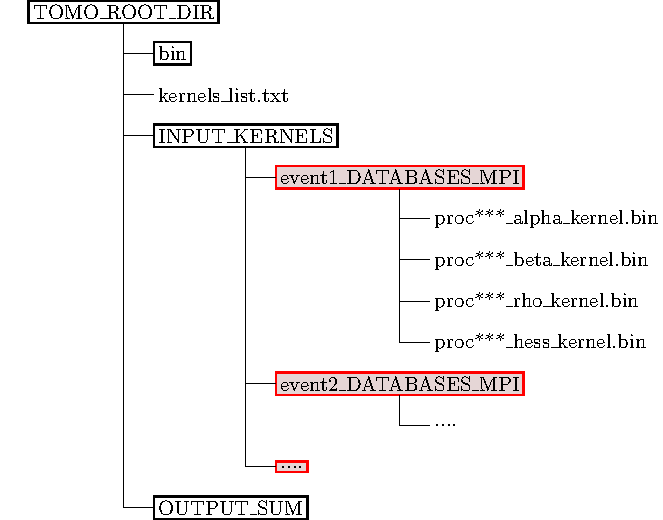
\includegraphics[width=4in]{figures/tomo_dir_struct.pdf}
\par\end{centering}
%
\caption{
Example directory structure when using tomographic tools for summation. Event directory names (red) can be chosen freely with corresponding name entries in file \texttt{kernels\_list.txt}}
\label{fig:tomo-dir-struct}
\end{figure}


\begin{description}
\item [Kernel summation:] As example with a total of 4 MPI processes
\begin{verbatim}
mpirun -np 4 ./bin/xsum_kernels
\end{verbatim}
adds sensitivity kernels $K$ from different events together, i.e. outputs $\boldg$ where
\begin{equation}
\boldg = \Sum^{N}_i K^{i} \nonumber
\end{equation}
for events $i = 1,..,N$ as specified in file \texttt{kernel\_list.txt}.

\item [Kernel Summation with Preconditioning:] As example with a total of 4 MPI processes
\begin{verbatim}
mpirun -np 4 ./bin/xsum_preconditioned_kernels
\end{verbatim}
adds sensitivity kernels $K$ together from different events and "preconditions" the sum by dividing with the sum of the corresponding approximate Hessians $\tilde{H}$, i.e. outputs $\boldg$ where
\begin{equation}
\boldg = \frac{1}{\Sum_i \tilde{H}^{i}} \; \Sum_i  K^{i} \nonumber
\end{equation}
In this case, the factor $\frac{1}{\Sum_i \tilde{H}^{i}}$ acts as preconditioner, approximating the inverse of the Hessian $\mathbf{H}^{-1}$.
\end{description}

\noindent
{\bf Kernel names}: The summation tool will look for kernels with following names:
\begin{itemize}
\item [-] for an {\it isotropic} model parameterization, kernel names are:\\
\begin{tabular}{ c c }
\begin{minipage}{3in}
\begin{verbatim}
## Cartesian version
proc***_alpha_kernel.bin
proc***_beta_kernel.bin
proc***_rho_kernel.bin
\end{verbatim}
\end{minipage}
&
\begin{minipage}{3in}
\begin{verbatim}
## GLOBE version
proc***_reg1_alpha_kernel.bin
proc***_reg1_beta_kernel.bin
proc***_reg1_rho_kernel.bin
\end{verbatim}
\end{minipage}
\end{tabular}\\

\item [-] for an {\it isotropic bulk} model parameterization, kernel names are:\\
\begin{tabular}{ c c }
\begin{minipage}{3in}
\begin{verbatim}
## Cartesian version
proc***_bulk_kernel.bin
proc***_bulk_beta_kernel.bin
proc***_rho_kernel.bin
\end{verbatim}
\end{minipage}
&
\begin{minipage}{3in}
\begin{verbatim}
## GLOBE version
proc***_reg1_bulk_kernel.bin
proc***_reg1_bulk_beta_kernel.bin
proc***_reg1_rho_kernel.bin
\end{verbatim}
\end{minipage}
\end{tabular}\\

\item [-] for a {\it transversely isotropic} model parameterization, kernel names are:\\
\begin{tabular}{ c c }
\begin{minipage}{3in}
\begin{verbatim}
## Cartesian version
proc***_bulk_c_kernel.bin
proc***_bulk_betav_kernel.bin
proc***_bulk_betah_kernel.bin
proc***_eta_kernel.bin
\end{verbatim}
\end{minipage}
&
\begin{minipage}{3in}
\begin{verbatim}
## GLOBE version
proc***_reg1_bulk_c_kernel.bin
proc***_reg1_bulk_betav_kernel.bin
proc***_reg1_bulk_betah_kernel.bin
proc***_reg1_eta_kernel.bin
\end{verbatim}
\end{minipage}
\end{tabular}\\

Note that these event kernels are stored after a kernel simulation (\texttt{SIMULATION\_TYPE = 3}) in the \texttt{LOCAL\_PATH} directory, which by default points to directory \texttt{DATABASES\_MPI/}. Isotropic kernels will be created by default. To create transversely isotropic kernels, you set \texttt{ANISOTROPIC\_KL} and \texttt{SAVE\_TRANSVERSE\_KL} to \texttt{.true.} in the parameter file \texttt{DATA/Par\_file}. \\

\item [- ] for preconditioning, the approximate Hessian kernels taken for summation are:\\
\begin{tabular}{ c c }
\begin{minipage}{3in}
\begin{verbatim}
## Cartesian version
proc***_hess_kernel.bin
\end{verbatim}
\end{minipage}
&
\begin{minipage}{3in}
\begin{verbatim}
## GLOBE version
proc***_reg1_hess_kernel.bin
\end{verbatim}
\end{minipage}
\end{tabular}\\

These Hessian kernels approximate the diagonal elements of the Hessian matrix and can be used as preconditioner in a gradient optimization scheme.
To create these kernels, you have to set \texttt{APPROXIMATE\_HESS\_KL} to \texttt{.true.} in the parameter file \texttt{DATA/Par\_file}.\\

\end{itemize}


For SPECFEM3D\_GLOBE, by default only kernels in the crust/mantle region ("reg1") will be considered for summation. You can change the default by setting parameter \texttt{REG} in file \texttt{constants\_tomography.h} to the region of interest. \\

Note that although we provide the preconditioned summation here, we recommend to smooth first both, the summed kernels and summed approximate Hessians, before inverting the summed Hessian and applying it as preconditioner to the gradient. From experience, we prefer doing
\begin{equation}
\boldg =  \frac{1}{\mathcal{F}_{smooth} \left( \Sum^{N}_i \tilde{H}^{i} \right) }  \; \mathcal{F}_{smooth} \left( \Sum_i K^{i}  \right) \nonumber
\end{equation}
rather than
\begin{equation}
\boldg = \mathcal{F}_{smooth} \left( \frac{1}{\Sum^{N}_i \tilde{H}^{i}}  \;  \Sum_i K^{i}  \right) \: . \nonumber
\end{equation}
Due to the large sensitivity kernel values close to source and receiver locations, the inverse of the thresholded summed Hessian becomes better balanced in the former.


\subsection{Smoothing and post-processing}
For additional smoothing and post-processing of kernels, gradients, or models, we provide tools useful for gradient and model preparation.
These additional tools for post-processing sensitivity kernels are provided together with the main package. For compilation of these tools, you type in the main directory:
\begin{verbatim}
make postprocess
\end{verbatim}

\noindent
The following tools are provided:
\begin{enumerate}
\item [-] \texttt{xsmooth\_sem} is used for smoothing with a gaussian function.
\item [-] \texttt{xclip\_sem} is used to threshold a kernel, gradient or model, clipping to a minimum and maximum value.
\item [-] \texttt{xcombine\_sem} is used to combine different event kernels, gradient or model files, summing all individually specified files together (similar to \texttt{xsum\_kernels} but more flexible).
\end{enumerate}
The post-processing tools are primarily intented to be used to process kernel files. They can be used though on
any scalar field of dimension \texttt{(NGLLX,NGLLY,NGLLZ,NSPEC)}.
The tools are parallel programs -- they must be invoked with mpirun or other
appropriate utility.  Operations are performed in embarrassingly-parallel fashion.



\begin{description}
\item [Smoothing:] To smooth a kernel, gradient or model file, use
\begin{verbatim}
mpirun -np NPROC bin/xsmooth_sem SIGMA_H SIGMA_V KERNEL_NAME INPUT_DIR OUPUT_DIR
\end{verbatim}
with command line arguments:
\texttt{SIGMA\_H} horizontal smoothing radius,
\texttt{SIGMA\_V} vertical smoothing radius,
\texttt{KERNEL\_NAME} kernel name, e.g. \texttt{alpha\_kernel},
\texttt{INPUT\_DIR} directory from which kernels are read,
\texttt{OUTPUT\_DIR} directory to which smoothed kernels are written.

Smooths kernels by convolution with a Gaussian. Writes the resulting
smoothed kernels to \texttt{OUTPUT\_DIR}.

Files written to \texttt{OUTPUT\_DIR} have the suffix 'smooth' appended,
e.g. \texttt{proc***alpha\_kernel.bin} becomes \texttt{proc***alpha\_kernel\_smooth.bin}.

\item [Clipping:] Values in a kernel, gradient or model binary file can be clipped with a minimum/maximum threshold value using
\begin{verbatim}
mpirun -np NPROC bin/xclip_sem MIN_VAL MAX_VAL KERNEL_NAMES INPUT_FILE OUTPUT_DIR
\end{verbatim}
with command line arguments:
\texttt{MIN\_VAL} threshold below which array values are clipped,
\texttt{MAX\_VAL} threshold above which array values are clipped,
\texttt{KERNEL\_NAMES} one or more kernel names separated by commas,
\texttt{INPUT\_DIR} directory from which arrays are read,
\texttt{OUTPUT\_DIR} directory to which clipped array are written.

For each name in \texttt{KERNEL\_NAMES}, reads kernels from \texttt{INPUT\_DIR}, applies
thresholds, and writes the resulting clipped kernels to \texttt{OUTPUT\_DIR}.

\texttt{KERNEL\_NAMES} is a comma-delimited list of kernel names,
e.g. \texttt{alphav\_kernel,alphah\_kernel}.
\begin{itemize}
\item [] For example, in this case type
{\small
\begin{verbatim}
mpirun -np 4 ./bin/xclip_sem -0.1 0.1 alphav_kernel,alphah_kernel DIR1/ DIR1/
\end{verbatim}
}
to clip the corresponding kernels in directory \texttt{DIR1} to be in range $[-0.1,0.1]$.
\end{itemize}

Files written to \texttt{OUTPUT\_DIR} have the suffix 'clip' appended,
e.g. \texttt{proc***alpha\_kernel.bin} becomes \texttt{proc***alpha\_kernel\_clip.bin}

\item [Combining:] To combine kernel values from different kernel directories, you can use
\begin{verbatim}
mpirun -np NPROC bin/xcombine_sem KERNEL_NAMES INPUT_FILE OUTPUT_DIR
\end{verbatim}
with command line arguments:
\texttt{KERNEL\_NAMES} one or more kernel names separated by commas,
\texttt{INPUT\_FILE} text file containing list of kernel directories,
\texttt{OUTPUT\_PATH} directory to which summed kernels are written.

For each name in \texttt{KERNEL\_NAMES}, sums kernels from directories specified in
\texttt{INPUT\_FILE}. Writes the resulting sums to \texttt{OUTPUT\_DIR}.

\texttt{INPUT\_FILE} is a text file containing a list of absolute or relative paths to
kernel directories, one directory per line.

\texttt{KERNEL\_NAMES} is a comma-delimited list of kernel names,
e.g. \texttt{alpha\_kernel,beta\_kernel,rho\_kernel}.



\end{description}

\subsection{Model updating}
We provide (simple) tools for updating the current model $\boldm_i$ using a gradient $\boldg$ and steplength $\alpha$:, i.e.
\begin{equation}
\boldm_{i+i} = \boldm_i + \delta \boldm  \nonumber
\end{equation}
with
\begin{equation}
\delta \boldm = - \alpha \, \boldg \nonumber \: .
\end{equation}
\noindent
The following tomographic tools are provided:
\begin{enumerate}
\item [-] \texttt{xadd\_model\_iso} can be used to update isotropic model files with a (summed \& smoothed) gradient.
The gradient files are given for isotropic parameters or isotropic bulk parameters.

\end{enumerate}

Note that instead of using the density kernels $K_{\rho}$ for model updates, setting \texttt{USE\_RHO\_SCALING} to \texttt{.true.} will
ignore the density kernel and use density perturbations scaled from isotropic $V_s$ pertubations.\\

\begin{description}
\item [Isotropic model update:] The program \texttt{xadd\_model\_iso} can be used to update {\it isotropic} model files with
(smoothed \& summed) event kernels:
\begin{verbatim}
mpirun -np 4 bin/xadd_model_iso step_factor [INPUT-KERNELS-DIR/] [OUTPUT-MODEL-DIR/]
\end{verbatim}
with command line arguments:
\texttt{step\_factor} the step length to scale the gradient, e.g. $0.03$ for a $\pm 3$\% update,
\texttt{INPUT-KERNELS-DIR/} (optional) directory which holds summed kernels (e.g. \texttt{proc***alpha\_kernel.bin},.., by default
directory \texttt{INPUT\_GRADIENT/} is used),
\texttt{OUTPUT-MODEL-DIR/} (optional) directory which will hold new model files (e.g. \texttt{proc***vp\_new.bin},.., by default directory
\texttt{OUTPUT\_MODEL/} is used).

The gradients are given for isotropic parameters \texttt{(alpha,beta,rho)} or \texttt{(bulk\_c,beta,rho)}.

The algorithm uses a steepest descent method with a step length
determined by the given maximum update percentage.

By default, the directory and file setup used is:
\begin{itemize}
\item [-] directory \texttt{INPUT\_MODEL/} contains:
\begin{verbatim}
proc***_vs.bin
proc***_vp.bin
proc***_rho.bin
\end{verbatim}

\item [-] directory \texttt{INPUT\_GRADIENT/} contains:
\begin{verbatim}
proc***_bulk_c_kernel_smooth.bin
proc***_bulk_beta_kernel_smooth.bin
proc***_rho_kernel_smooth.bin
\end{verbatim}
or
\begin{verbatim}
proc***_alpha_kernel_smooth.bin
proc***_beta_kernel_smooth.bin
proc***_rho_kernel_smooth.bin
\end{verbatim}
depending on the model parameterization.

\item [-] directory \texttt{topo/} contains:
\begin{verbatim}
proc***_external_mesh.bin
\end{verbatim}
for the Cartesian version, and
\begin{verbatim}
proc***_solver_data.bin
\end{verbatim}
for the GLOBE version.
\end{itemize}

\noindent
The new model files are stored in directory \texttt{OUTPUT\_MODEL/} as
\begin{verbatim}
proc***_vp_new.bin
proc***_vs_new.bin
proc***_rho_new.bin
\end{verbatim}

\end{description}

Note that additional post-processing and model update tools are provided for the SPECFEM3D\_GLOBE version and will be provided for the Cartesian version as well in future.


\section{OLD VERSION OF THE SECTION, WILL SOON BE IMPROVED AND ENRICHED}

There are many other versions of gradient-based inversion
algorithms that could alternatively be used (see e.g. \cite{ViOp09,MoChKoWa15} for a list).
The tomographic inversion of \citet{TaLiMaTr09,TaLiMaTr2010} used SPECFEM3D\_Cartesian as well
as several additional components which are also stored on the CIG
svn server, described next.

The directory containing external utilities for tomographic inversion using
SPECFEM3D Cartesian (or other packages that evaluate misfit functions
and gradients) is in directory \texttt{utils/ADJOINT\_TOMOGRAPHY\_TOOLS/}:
\begin{verbatim}
flexwin/     -- FLEXWIN algorithm for automated picking of time windows
measure_adj/ -- reads FLEXWIN output file and makes measurements,
                with the option for computing adjoint sources
iterate_adj/ -- various tools for iterative inversion
                (requires pre-computed "event kernels")
\end{verbatim}
This directory also contains
a brief \verb+README+ file indicating the role of the three subdirectories,
\verb+flexwin+ \citep{Maggi2009}, \verb+measure_adj+, and \verb+iterate_adj+.
The components for making the model update are there; however, there
are no explicit rules for computing the model update, just as with
any optimization problem. There are options for computing a conjugate
gradient step, as well as a source subspace projection step.

The best single file to read is probably: \verb+ADJOINT_TOMO/iterate_adj/cluster/README+.


